\chapter{Architektur des WCCS}
    Abbildung \ref{image:wccsExternalArchitecture} zeigt die vollständige Architektur des \glspl{wccs},
    wie sie in Kapitel \ref{section:Architecture} vorgestellt wurde.

    \begin{figure}[htb]
        \centering
        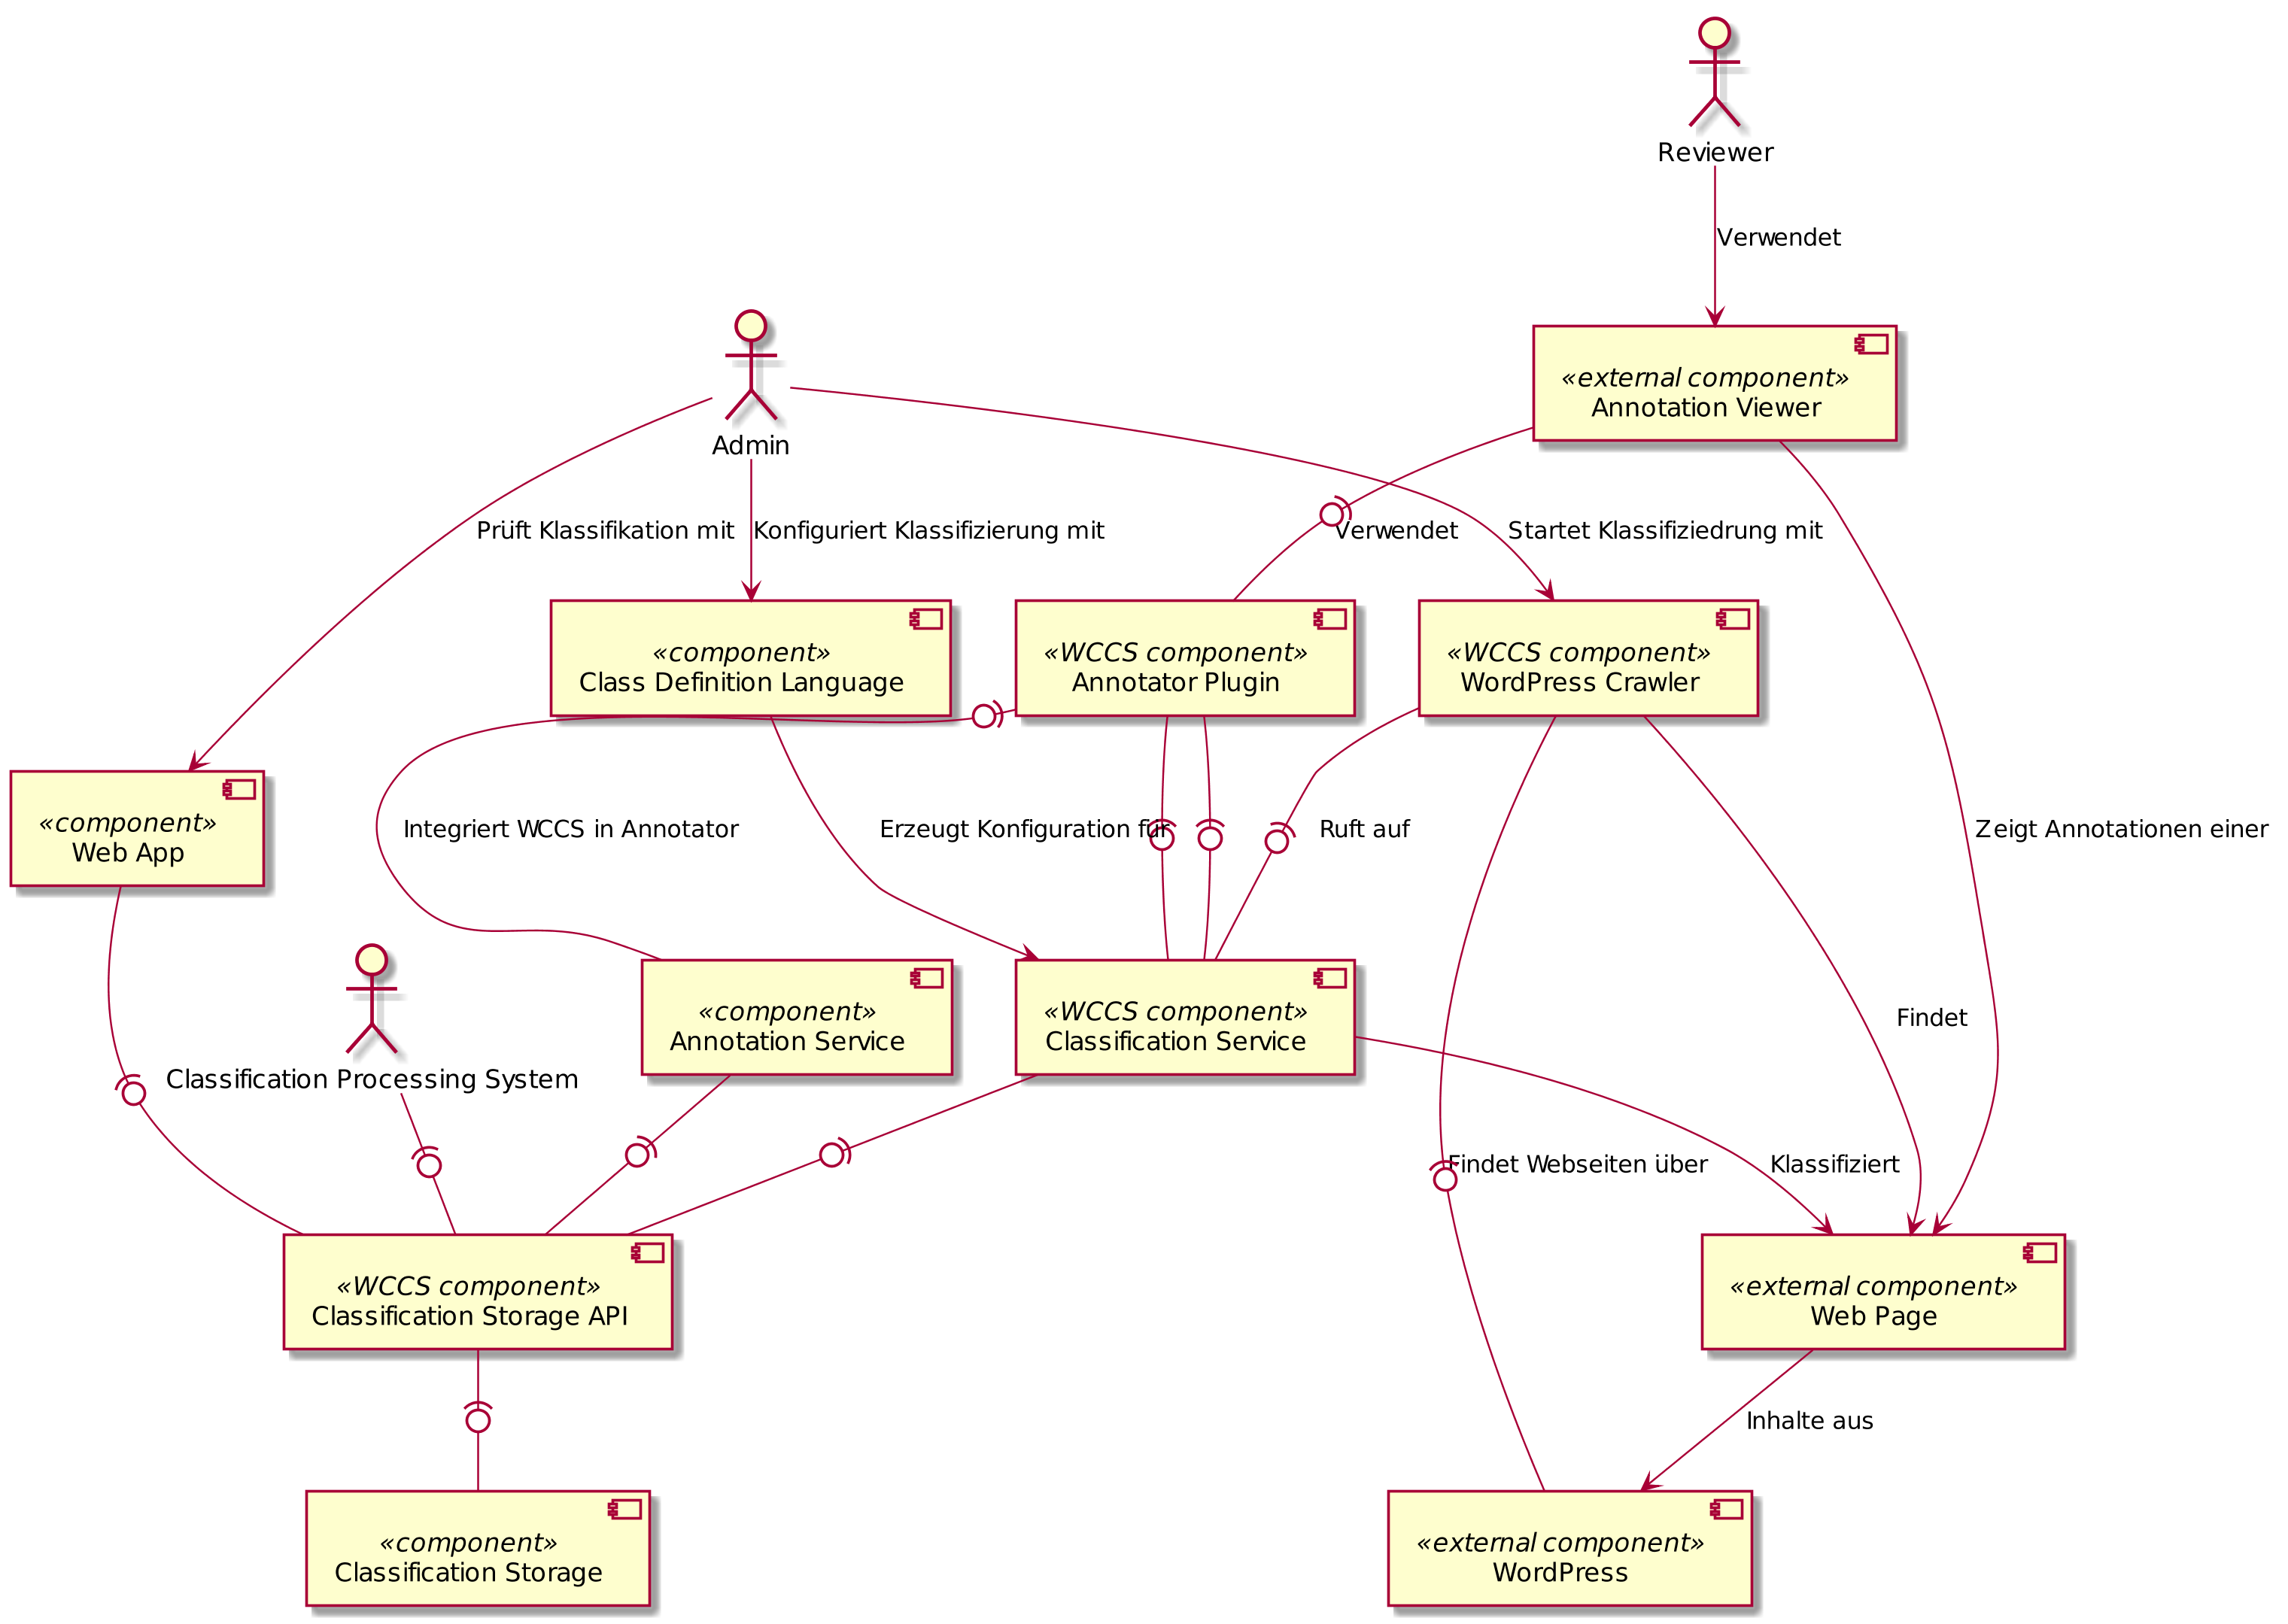
\includegraphics[width=\textwidth]{../resources/architecture/complete_architecture.png}
        \caption{Architkektur des \glspl{wccs}}
        \label{image:wccsExternalArchitecture}
    \end{figure}

\chapter{DSL}
    \section{Modell}
        \begin{figure}[htb]
            \centering
            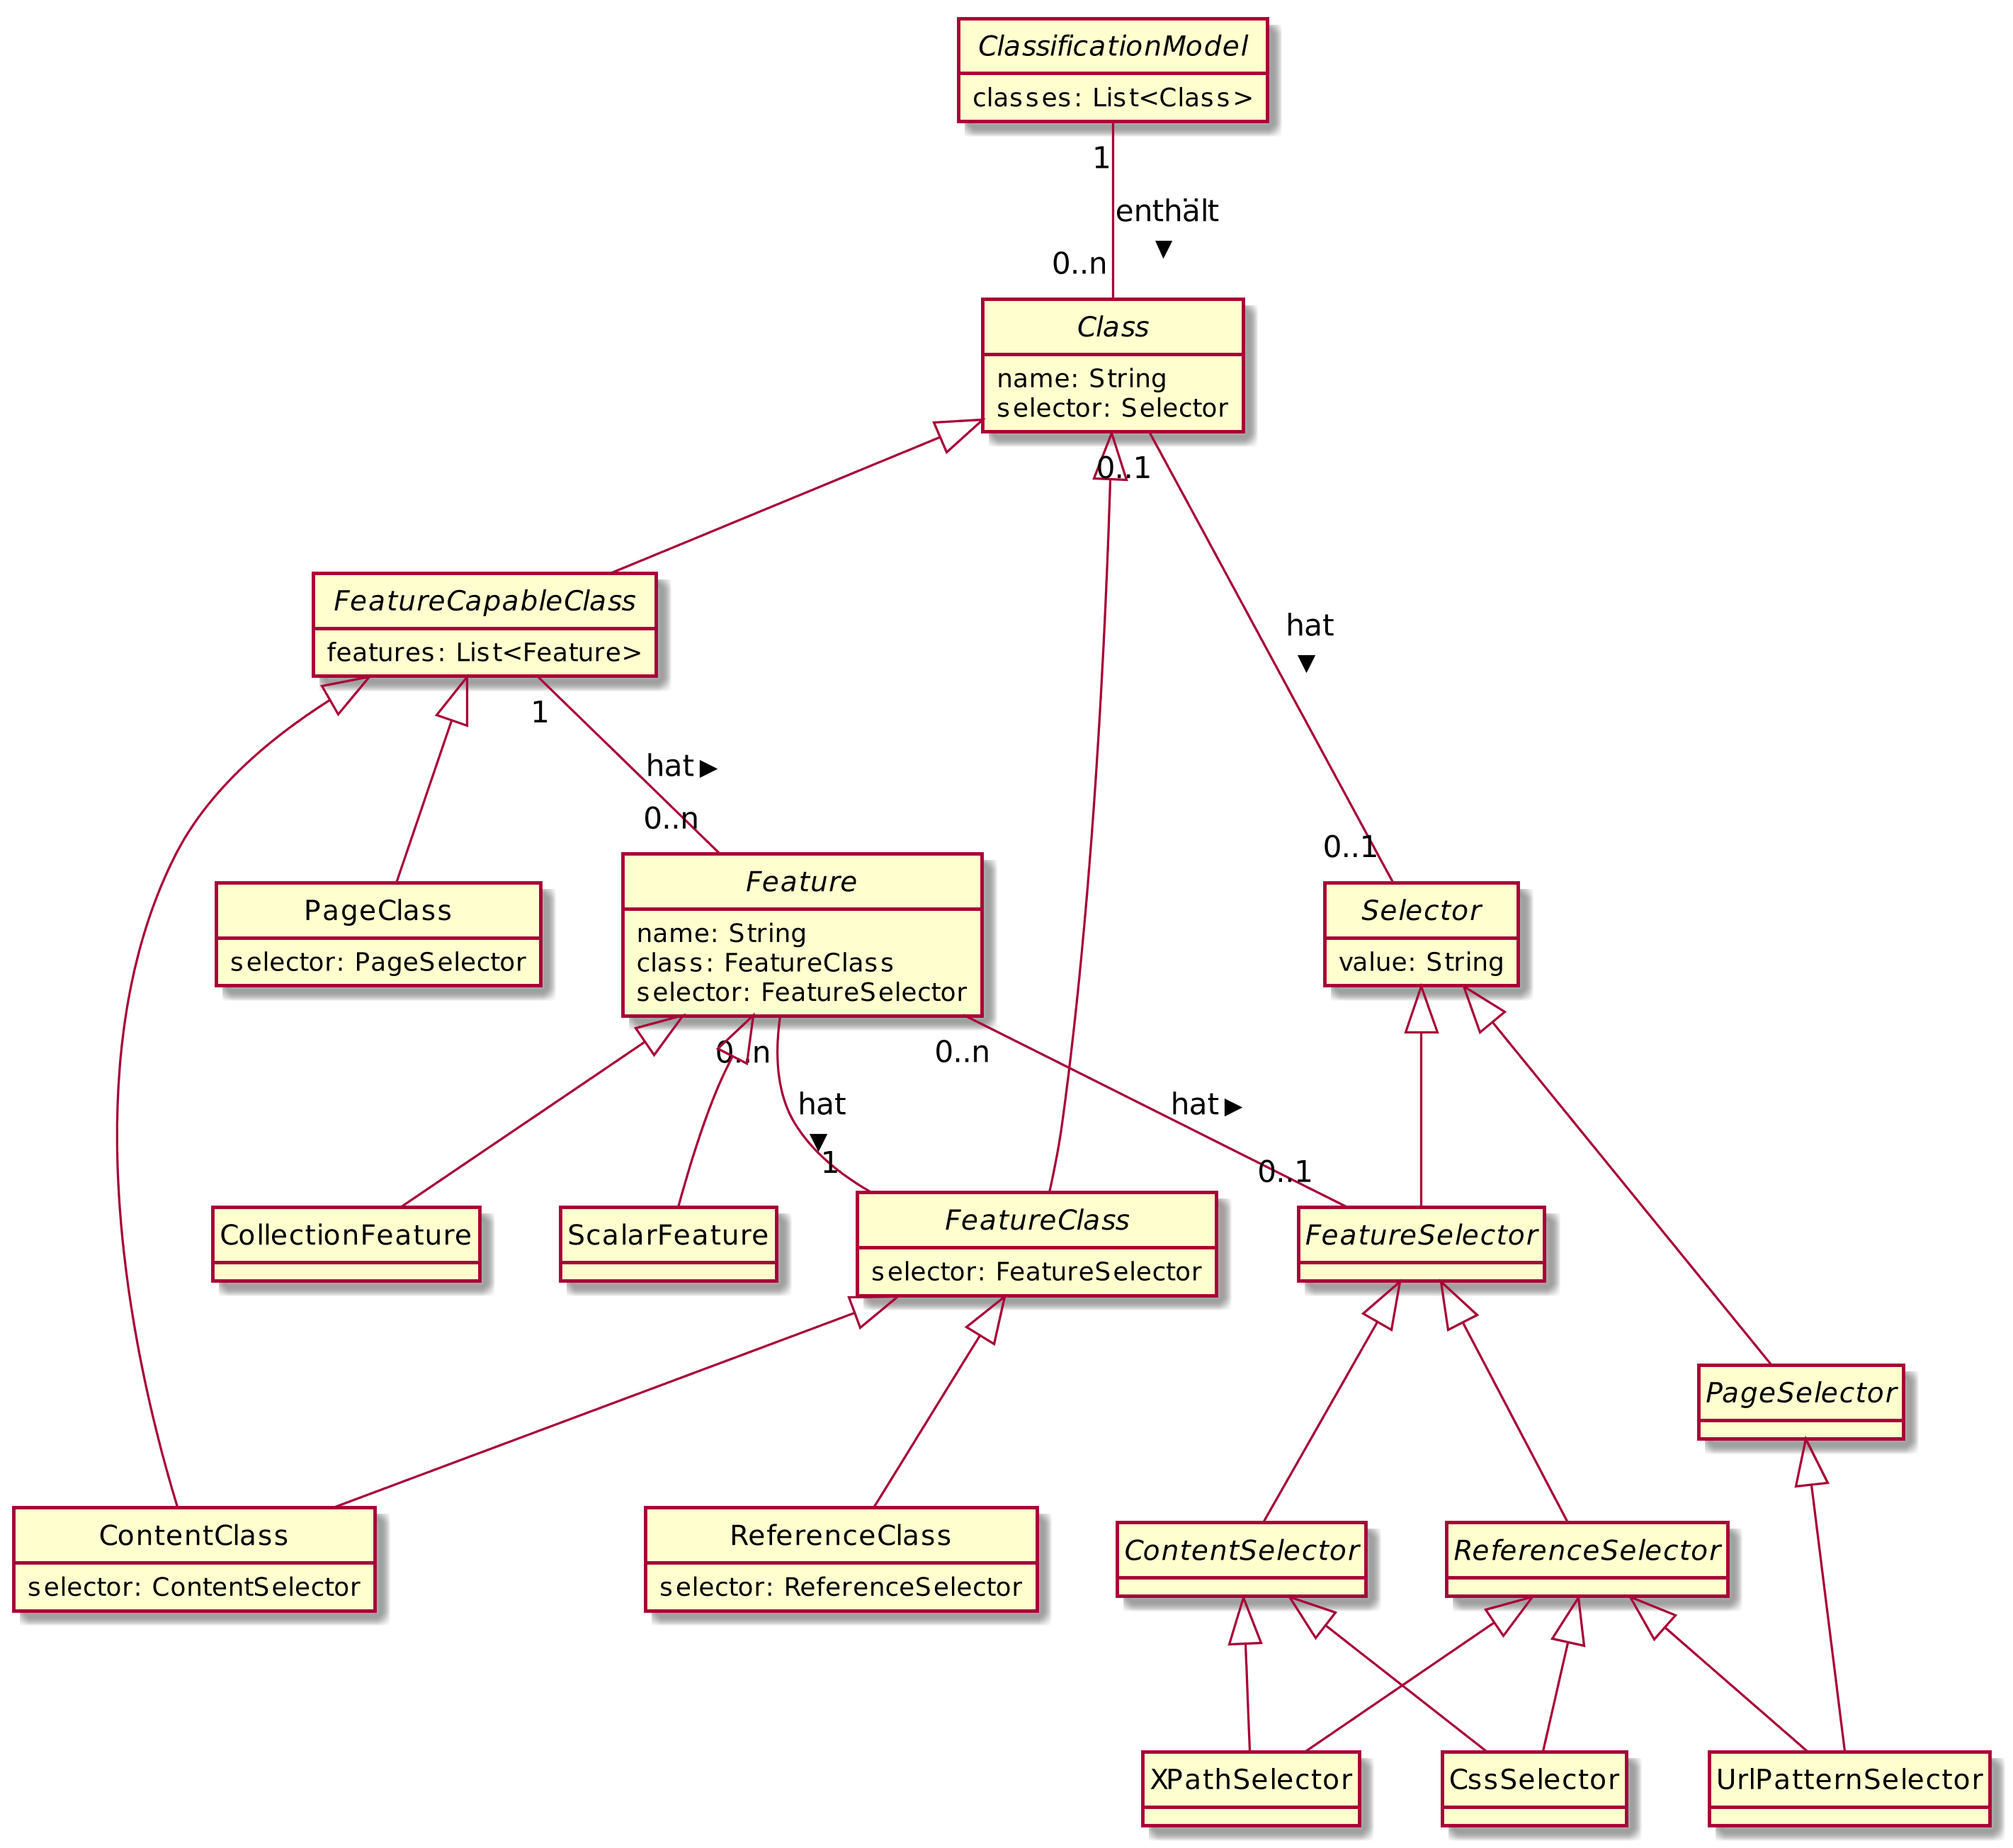
\includegraphics[width=\textwidth]{../resources/dsl/model.png}
            \caption{Modell der DSL}
            \label{image:dslCompleteModel}
        \end{figure}
    
    \section{Grammatik}
        \lstinputlisting[
            label=listing:dlsGrammar,
            caption=Grammatik der DSL,
            language=wccdl,
            inputencoding=utf8/latin1]{../resources/dsl/grammar/grammar.xtext}

    \section{Transformation}
    \lstinputlisting[label=listing:dlsGenerationComplete,caption=Vollständiges Generat]{../resources/dsl/generation/complete.js}